\section{Riduzioni polinomiali}
Si hanno alcuni problemi che sono in grado di risolvere qualunque problema di decisione in \textbf{NP}. Serviranno prima le definizioni di \textbf{NP-difficili} e \textbf{NP-complete}.\\
\subsection{Indipendent-Set}
L'\textit{independent-set } di un grafo non orientato è un sottoinsieme $I\subseteq V$ tale che $\forall u,v\in I$ $(u,v)\notin E$. 
Il problema \textit{ind\_set}, nella versione di ottimo ha come questione di trovare l'\textit{independent-set} di cardinalità massima di un grafo non orientato. Nella versione di decisione $ind\_set_d$ si ha anche il parametro $k$ intero e si cerca se esiste un \textit{independent-set} di cardinalità uguale a $k$. L'\textit{independent-set} di cardinalità massima può essere usato come certificato.

La relazione che si ha tra copertura di $V'$ di G e l'insieme indipendente di G. Sapendo che la copertura $V' \subseteq V$ | $\forall \, e = (u,v) \in E$ almeno un estremo di $e$ è in $V'$. $V - V' = I$ con $V'$ copertura minima e $I$ massimo insieme indipendente. Il complemento di una copertura è un insieme indipendente.


\subsection{Dimostrazione del Indipendent Set}
Come faccio a dimostrare che il problema $ind\_set_d \in$ NP?

$\exists$ un algoritmo $A$ che ha costo polinomiale in tempo e che dato in input $x=(G,k)$ e un certificato $y$ (che corrisponde ai vertici di un insieme indipendente di dimensione $k$). \\ Se noi sappiamo che un algoritmo prende in input $x, y$, allora è in grado di verificare sul grafo $G$ che $y$ è un insieme indipendente. \\
L'algoritmo verifica che $y$ è un \textit{independent-set} e il costo della verifica è quadratico su $|y|$, ovvero $|y|^2$ che nel caso peggiore è $|V|^2$. So anche che, per l'input $x$, $O(|x|)=O(|E|+|V|)=O(|V^2|+|V|)$ nel caso peggiore, quindi il tempo di verifica è \textbf{quadratico}.

\subsection{SAT - satisfiability}
Il problema di \textbf{soddisfacibilità} $SAT$, è un problema che prende in input una formula booleana $\phi$ in \textbf{forma normale congiunta (CNF)}, ovvero che ha una congiunzione ($\land$) come legame tra le \textbf{clausole}. Una clausola è un $\lor$ di \textbf{letterali}, ovvero di variabili booleane $x_i$ o $\neg x_i$. In output ho se la forma sia soddisfacibile o meno.\\

La complessità dei problemi di decisione SAT è legata a un parametro $k-SAT$ che rappresenta il numero letterali che compongono la clausola. Si ha che $2SAT\in P$ ma con $k>2$ si ha che $k-SAT\in NP$ (in realtà è in \textbf{NP-difficili})

\subsection{Problema NP-difficile}
Un problema del genere è un problema più difficile in NP, ovvero almeno difficile quanto ogni altro problema in NP. Sia $B$ un problema NP-difficile, ogni problema $A$ che sta in NP può essere risolto con una chiamata di procedura a $B$, quindi effettuando una riduzione. \\
\begin{figure}[H]
    \centering
    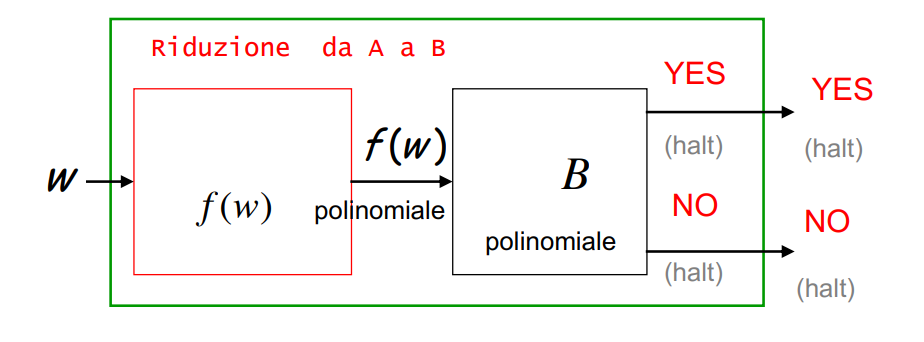
\includegraphics[scale = 0.5]{imm/riduzione.PNG}
    \label{fig:my_label}
\end{figure}
Ad esempio, vertex-cover è NP-difficile, questo significa che posso risolvere ogni problema $A$ in NP con il problema vertex-cover $B$. Per fare questo, si trasforma l’input $w$ di $A$ in un input $f(w)$ per $B$ in tempo polinomiale. La risposta di $B$ con input $f(w)$ è la stessa che $A$ da su input $w$.
\newline
\textbf{UN PROBLEMA NP-DIFFICILE NON è DETTO CHE STIA DENTRO I PROBLEMI DI TIPO NP, NEL CASO IN CUI STIA DENTRO NP ALLORA POSSIAMO DIRE CHE è NP-COMPLETO}

\subsubsection{Riduzione polinomiale da A a B}
Consiste nel trasformare l’input $w$ di $A$ in un input $f(w)$ per $B$ in tempo polinomiale (il calcolo di $f(w)$ è $\mathcal{O} (|w|^p)$). La risposta di $B$ con input $f(w)$  è la stessa che $A$ da su input $w$.
Si ha che $A$ si riduce polinomialmente a $B$, e si scrive: $A\leq_p B$ se $\exists \ f$ tale che: $w \in L_A\mbox{ sse } f(w)\in L_B$ con $f$ calcolabile in tempo polinomiale.

\subsubsection{Definizione di NP-difficile}
Avevamo detto che ogni problema $A$ che in \textbf{NP} può essere risolto con una chiamata di procedura a $B$, quindi posso risolvere ogni problema $A\in NP$ con \textit{vertex-cover}, essendo esso un problema \textbf{NP-difficili}, ma cosa sono i problemi NP-difficili?

Un problema $B$ è NP-difficile se e solo se $\forall \, A \in NP$ , $A$ si riduce a $B$ in tempo polinomiale, cioè $A \leq_p B$.

Un problema $NP-difficili$ può non essere in $NP$, in quanto potrebbe non avere un certificato (y) per consentire la verifica in tempo polinomiale. \\ 
Un problema \textbf{NP-difficili} e anche \textbf{NP} si dice che il problema è \textbf{NP-complete}. Sappiamo inoltre che $SAT$ è il primo problema che si è dimostrato essere anche \textbf{NP-complete}.

Esistono problemi NP-difficili non in NP.

\begin{enumerate}
    \item SAT è il primo problema che si è dimostrato essere NP-completo.
    \item 3-SAT $\leq_p$ IND-SET
    \item IND-SET è NP-completo
\end{enumerate}

$\phi_w$ è soddisfacibile sse $G_\phi$ (che rappresenta $f(w)$) ha un IND-SET di dimensione $k=|\phi| = $ numero di clausole della formula.

Data una istanza $\phi$ di 3-SAT, costruiamo una istanza $(G, k)$ di IND-SET che ha un insieme indipendente di dimensione $k$ sse $\phi$ è soddisfacibile. 
Per farlo si costruisce un grafo $G$ che contiene 3 vertici per ogni clausola, uno per ogni letterale della clausola. In seguito collego i 3 letterali di una clausola con un triangolo (formando un gadget) e si collega ogni letterale al suo negato.
\begin{figure}[H]
    \centering
    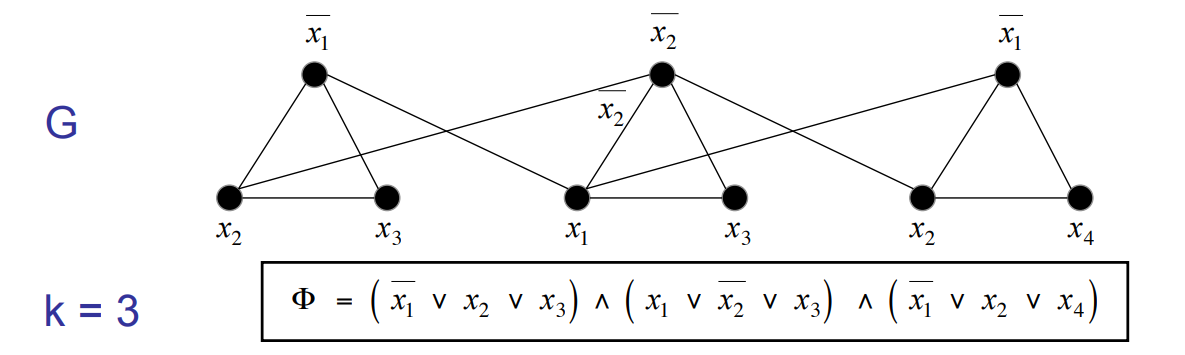
\includegraphics[scale = 0.5]{imm/g-3.PNG}
    \label{fig:my_label2}
\end{figure}